\section{Remote sensing}


\subsection{Electromagnetic radiation}
Satellites all work the same way: they are flying machines that carry a camera. The camera has one or more sensors, each of which can observe some part of the electromagnetic spectrum.
Radar satellites (usually) additionally have their own 'light' source: they actively send out radio-radiation and collect the reflection.

\begin{itemize}
    \item Optical
    \item Radar: not hindered by clouds. Good for flood-detection
\end{itemize}





\subsection{Orbital periods and acquisition}
Satellites usually have an orbital period of 1 - 2 hours. They revisit the same spot on earth every 2-3 weeks.
(This example data is taken from landsat: an orbit takes 99 minutes, and it visits the same spot every 16 days.
Note that landsat always stays on the sunny side of earth - most visible-light satellites do this.)
Commonly, satellite series have offset periods so one machine of the same series
visits the same spot every nth of a full orbital period.
However, some satellites can narrow or broaden their sensors, so even if
a satellite visits the same spot again, it might not make the same snapshot again.
To handle the high demand and low availability of satellite images, acquisition plans are being made.
Usually, these take into account seasonal effects,
water vapor, and also a ranking of requests from different scientific institutions.








\subsection{Important satellites and service providers}


\begin{table}
    \centering
    \begin{tabular}{llllllll}
        \toprule
        Satellite   & Owner & Bands & Data available at                    & Started    & Orbit                                                         & Resolution & Description                                               \\
        \midrule
        Landsat     & NASA  &       & USGS Earth explorer / AWS-S2 as COGs &            &                                                               &            & US optical, very long running                             \\
        Modis       & NASA  &       &                                      &            &                                                               &            & Optical (but very coarse) / Temperature, water-vapor      \\
        Copernicus  & ESA   &       &                                      &            &                                                               &            &                                                           \\
        Sentinel 1  & ESA   &       & Sentinel-hub EO-browser              & 03.04.2014 & Near-polar, sun-sync, 1.5h, 6-day world coverage (using both) & 5m * 5m    & Radar                                                     \\
        Sentinel 2  & ESA   &       & Sentinel-hub EO-browser              &            &                                                               &            & Optical                                                   \\
        Sentinel 3  & ESA   &       & Sentinel-hub EO-browser              &            &                                                               &            & Sea surface topography, temperature (also fire detection) \\
        Sentinel 5p & ESA   &       & Sentinel-hub EO-browser              &            &                                                               & 6km * 4km  & Atmospheric gasses                                        \\
        TerraSarX   & DLR   &       &                                      & 15.06.2007 &                                                               & 1m/3m/16m  & Radar, very high resolution, commercial/scientific coop   \\
        RapidEye    &       &       &                                      &            &                                                               &            &                                                           \\
        Ikonos      &       &       &                                      &            &                                                               &            &                                                           \\
        \bottomrule
    \end{tabular}
\end{table}

\paragraph{Landsat} program is the longest-running enterprise for acquisition of satellite imagery of Earth. On July 23, 1972 the Earth Resources Technology Satellite was launched. This was eventually renamed to Landsat.[1] The most recent, Landsat 8, was launched on February 11, 2013. The instruments on the Landsat satellites have acquired millions of images. The images, archived in the United States and at Landsat receiving stations around the world, are a unique resource for global change research and applications in agriculture, cartography, geology, forestry, regional planning, surveillance and education, and can be viewed through the U.S. Geological Survey (USGS) 'EarthExplorer' website. Landsat 7 data has eight spectral bands with spatial resolutions ranging from 15 to 60 meters; the temporal resolution is 16 days.[2] Landsat images are usually divided into scenes for easy downloading. Each Landsat scene is about 115 miles long and 115 miles wide (or 100 nautical miles long and 100 nautical miles wide, or 185 kilometers long and 185 kilometers wide).

\paragraph{Modis} ...

\paragraph{Copernicus} ...

\paragraph{Sentinel} ESA is currently developing seven missions under the Sentinel programme. The Sentinel missions include radar and super-spectral imaging for land, ocean and atmospheric monitoring. Each Sentinel mission is based on a constellation of two satellites to fulfill and revisit the coverage requirements for each mission, providing robust datasets for all Copernicus services.

\paragraph{CHIRPS} is ...

\paragraph{EODC}: \href{https://www.eodc.eu/}{Earth Observation Data Center for Water Resources Monitoring}

\paragraph{Eurac}: \href{http://www.eurac.edu}{Eurac} is a private research company ...

\paragraph{Google Earth Engine} provides ...

\paragraph{NASA's ECS} (Earth observation center Core System) is a vast catalogue of ...






\subsection{Datatypes, protocols and libraries}

Remote sensing data is usually massive in size and requires some special software to parse.
This section is intended to give an overview of the different data-types out there and the tools for reading them.

\paragraph{Datacubes} are tensors of (usually very large) (geo-)data.

\paragraph{OGC-WCPS: OGC's Web Coverage Processing Service} is a language for filtering and processing multi-dimensional raster coverages.

\paragraph{Open-EO} ia an API to speak to different geo-processing services like GEE. Unfortunately, open-EO stands in concurrence to WCPS.

\paragraph{geoTiff} files are geo-referenced images. They contain different bands.
Every band is a 2d-array of 16-bit numbers, representing the image at one frequency-band.
Usually, you'll have one band around the green color, one around the red, and one around the blue (plus many more bands at non-visible frequencies).
When you color these three bands and put them together as an rgb-image, you can usually obtain a quite decent color-photo.
Every geoTiff has an associated \include{transform} attribute. This attribute is an affine transformation matrix and maps pixel-locations (row,col) to (x,y) spatial positions.
\begin{lstlisting}[language=python]
import rasterio

with rasterio.open("example.tif") as dataset:
    print(dataset.crs)
    print(dataset.transform)
    print(dataset.transform * (0, 0))
    print(dataset.transform * (dataset.width, dataset.height))
\end{lstlisting}

\paragraph{GeoPackage} (GPKG) is an open, non-proprietary, platform-independent and standards-based data format for geographic information system implemented as a SQLite database container.
Defined by the Open Geospatial Consortium (OGC)[1] with the backing of the US military[2] and published in 2014, GeoPackage has seen wide widespread support from various government,
commercial, and open source organizations[3].








\subsection{Projections}

\paragraph{Wgs84 aka. Epsg4326} is a global spherical (aka non-projected, using lat/lon) CRS and the stuff that comes from GPS-satellites. GeoJson should by now only  use Wgs84 in its data (it used to be allowed to add a field named "crs").
\paragraph{UTM aka. Epsg20**} is a projected CRS using a  two-dimensional cartesian grid in meters. Projections needs to be done on individual areas, which is why there several Epsg-codes for this projection.
\paragraph{Web Merkator aka. EPSG:900913 aka. Epsg3857} is the google projection and a variant of UTM.






\subsection{NDVI}
The normalized difference vegetation index (NDVI) is used to assess the state of vegetation. In living plants chlorophyll-A, from the photosynthetic machinery, strongly absorbs red color; on the other hand, near-infrared light is strongly reflected. Live, healthy vegetation reflects around 8% of red light and 50% of near-infrared light. Dead, unhealthy, or sparse vegetation reflects approximately 30% of red light and 40% of near-infrared light.
The NDVI is calculated as:
$$ NDVI = \frac{\lambda_{NIR} - \lambda_{red}}{\lambda_{NIR} + \lambda_{red}} $$
where:
\begin{itemize}
    \item $\lambda_{NIR}$ is near-infrared Band 5
    \item $\lambda_{red}$ is color red Band 4
\end{itemize}
By its formulation, NDVI ranges from -1 to +1. In practice, an area of an image containing living vegetation will have NDVI in the range 0.3 to 0.8. High water content clouds and snow will have negative values of the index. Bodies of water, having low reflectance in both Band 4 and 5, exhibit very low positive or negative index. Soil, having slightly higher reflectance in near-infrared than in red, will produce low positive values of the index.

Calculation of the NDVI is sensitive to to a few factors:
\begin{itemize}
    \item Atmospheric composition and appropriate modeling influence the calculation, especially if the correct water and aerosol content are initially incorrectly estimated.
    \item Thin, hard to spot clouds like cirrus can significantly affect the calculation.
    \item Sensor effects such as Sun angle not being calculated on per-pixel basis can influence the index estimation.
\end{itemize}



\subsection{Image (co-)registration}
Image registration is the process of transforming different sets of data into one coordinate system.

\begin{figure}[H]
    \centering
    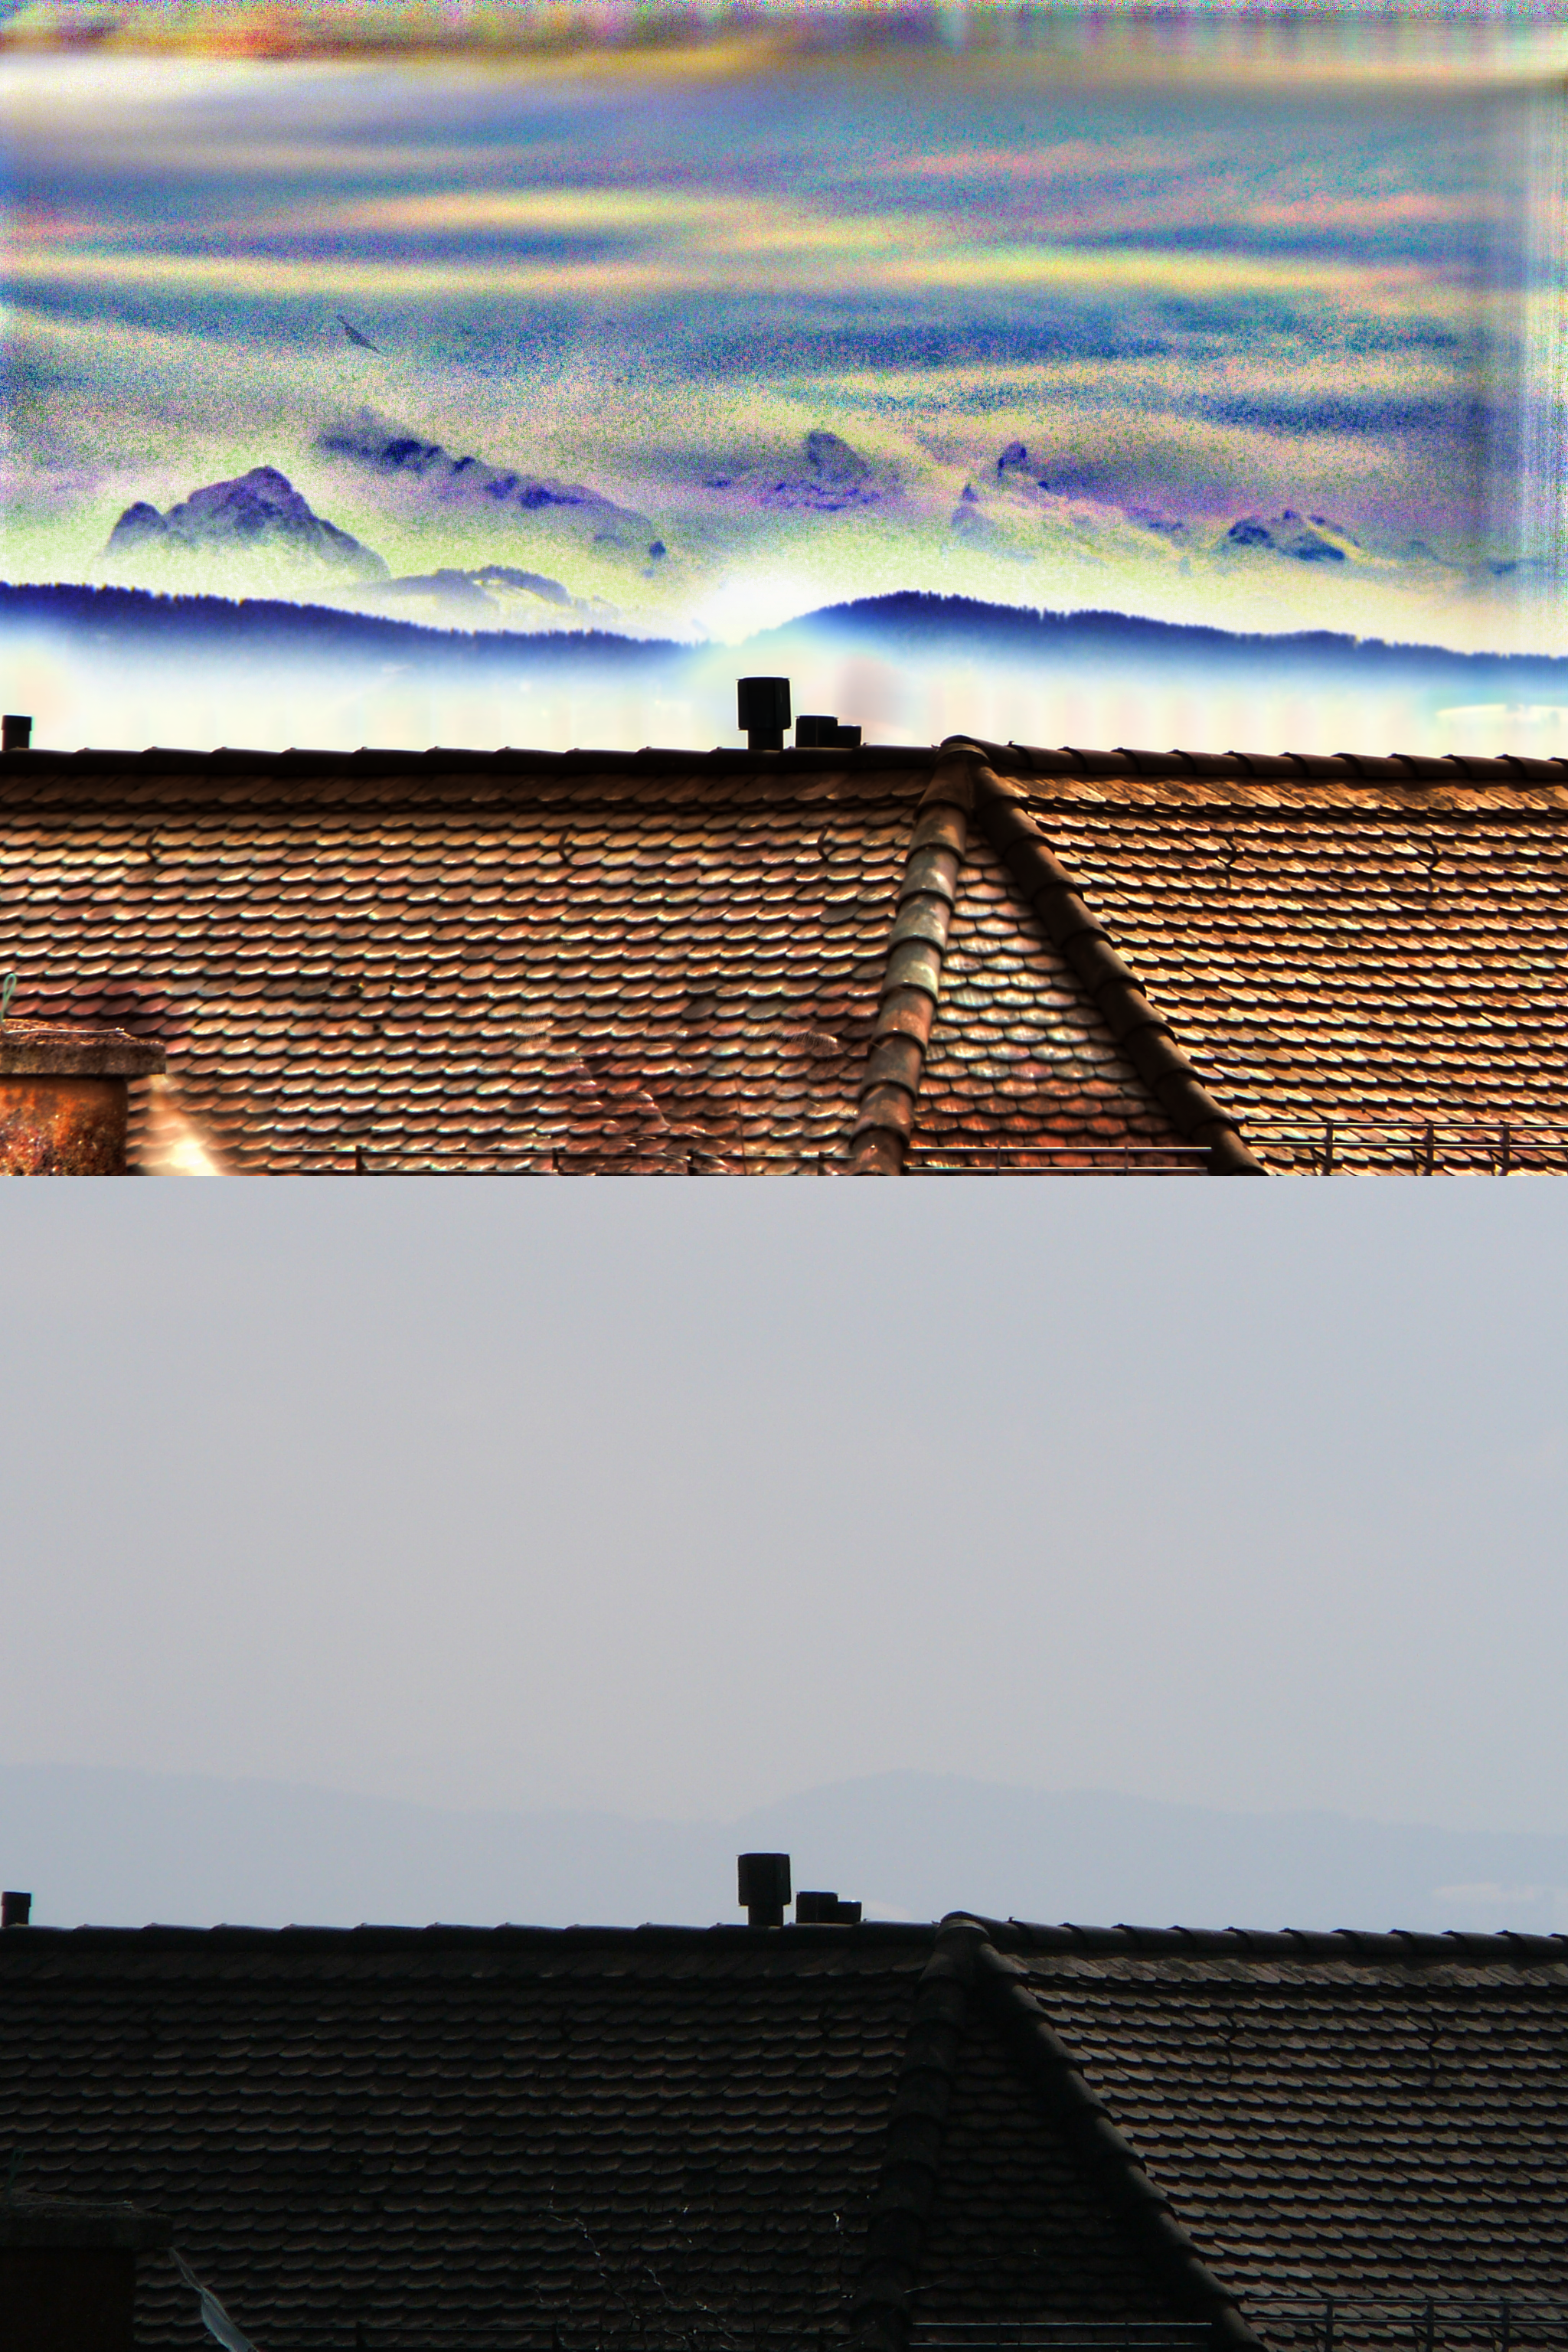
\includegraphics[width=0.5\textwidth]{images/imageRegistration.png}
    \caption{Registering and summing multiple exposures of the same scene improve signal to noise ratio, allowing one to see things previously impossible to see. In this picture, the distant Alps are made visible, although they are tens of kilometers into the haze.}
\end{figure}